\documentclass[tikz,border=6pt]{standalone}
\usepackage[T1]{fontenc}
\usepackage[utf8]{inputenc}
\usepackage{pgfplots}
\usepgfplotslibrary{groupplots}
\usetikzlibrary{calc}
\pgfplotsset{compat=1.18}
\begin{document}
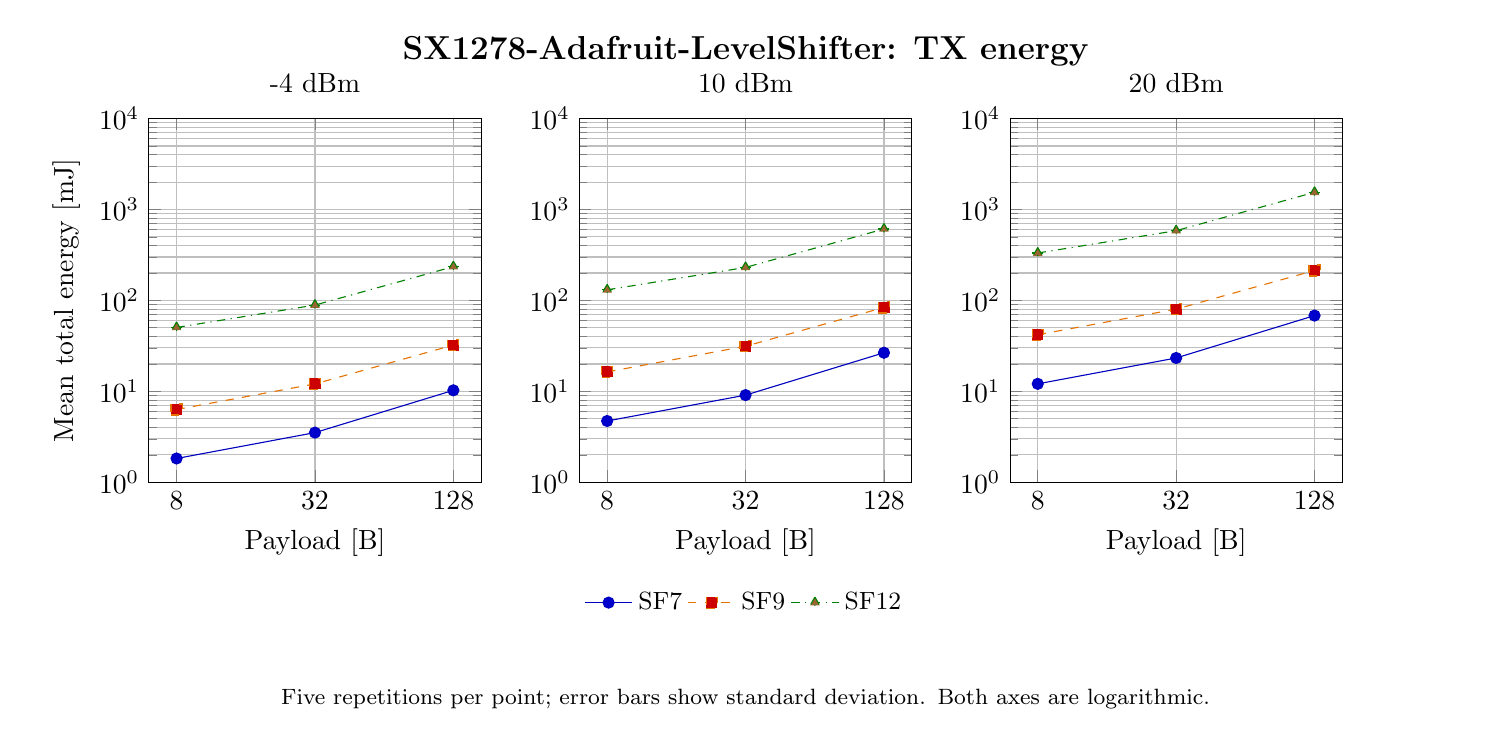
\begin{tikzpicture}
\begin{groupplot}[/pgf/number format/use comma, group style={group size=3 by 1, horizontal sep=1.25cm},
  width=5.8cm,height=6.2cm,xmode=log,log basis x=2,ymode=log,log basis y=10,ymin=1,ymax=10000,
  xtick={8,32,128},xticklabels={8,32,128},grid=both,xlabel={Payload [B]},
  legend style={draw=none,fill=none,font=\small,at={(0.5,-0.27)},anchor=north,legend columns=-1}]
% TX energy
\nextgroupplot[title={-4 dBm},ylabel={Mean total energy [mJ]}]
\addplot+[blue!75!black,solid,mark=*,error bars/.cd,y dir=both,y explicit] coordinates {(8,1.82465019) +- (0,0.00135166925) (32,3.51379398) +- (0,0.00640487752) (128,10.2560203) +- (0,0.00993246382)};
\addplot+[orange!90!black,dashed,mark=square*,error bars/.cd,y dir=both,y explicit] coordinates {(8,6.31026483) +- (0,0.00908979757) (32,12.0637686) +- (0,0.0166059317) (128,32.253423) +- (0,0.0315476641)};
\addplot+[green!50!black,dashdotted,mark=triangle*,error bars/.cd,y dir=both,y explicit] coordinates {(8,50.4147067) +- (0,0.0562340152) (32,88.8251087) +- (0,0.0563815705) (128,235.145251) +- (0,0.224299633)};
\nextgroupplot[title={10 dBm}]
\addplot+[blue!75!black,solid,mark=*,error bars/.cd,y dir=both,y explicit] coordinates {(8,4.71662276) +- (0,0.00309294877) (32,9.07927494) +- (0,0.0028348438) (128,26.562296) +- (0,0.0125106997)};
\addlegendentry{SF7}
\addplot+[orange!90!black,dashed,mark=square*,error bars/.cd,y dir=both,y explicit] coordinates {(8,16.341189) +- (0,0.0119708799) (32,31.3166251) +- (0,0.0208332802) (128,83.6737473) +- (0,0.0200397251)};
\addlegendentry{SF9}
\addplot+[green!50!black,dashdotted,mark=triangle*,error bars/.cd,y dir=both,y explicit] coordinates {(8,130.681012) +- (0,0.0353598242) (32,230.546356) +- (0,0.124175096) (128,610.508351) +- (0,0.331100235)};
\addlegendentry{SF12}
\nextgroupplot[title={20 dBm}]
\addplot+[blue!75!black,solid,mark=*,error bars/.cd,y dir=both,y explicit] coordinates {(8,12.0833452) +- (0,0.028895927) (32,23.2650379) +- (0,0.0774560086) (128,68.085163) +- (0,0.139433966)};
\addplot+[orange!90!black,dashed,mark=square*,error bars/.cd,y dir=both,y explicit] coordinates {(8,41.90498) +- (0,0.0887020748) (32,80.2100609) +- (0,0.243183189) (128,213.336994) +- (0,0.665267478)};
\addplot+[green!50!black,dashdotted,mark=triangle*,error bars/.cd,y dir=both,y explicit] coordinates {(8,332.076728) +- (0,0.32096582) (32,584.941586) +- (0,0.445553609) (128,1546.35068) +- (0,0.895340497)};
\end{groupplot}
\node[font=\bfseries\large] at ($(group c2r1.north)+(0,0.85cm)$) {SX1278-Adafruit-LevelShifter: TX energy};
\node[font=\footnotesize,align=center,text width=18cm] at ($(group c2r1.south)+(0,-2.75cm)$) {Five repetitions per point; error bars show standard deviation. Both axes are logarithmic.};
\end{tikzpicture}
\end{document}
